\documentclass[10pt,openright,twoside,french]{book}

\input philippe2013
\input philippe2013_cours
\input philippe2013_sections
\input philippe2013_chapitre
\renewcommand\PartProgramme{Géométrie}
\renewcommand\MaCouleur{Purple}

\pieddepage{}{%
\begin{tikzpicture}[scale=0.65]
\shadedraw [top color=white, bottom color=\MaCouleur, draw=\MaCouleur]
[l-system={Sierpinski triangle, step=1pt, angle=60, axiom=F, order=6.5}]
lindenmayer system -- cycle;
\draw (30:0.65cm) node {\bfseries\textcolor{black}{\thepage}};
\end{tikzpicture}%
}{}


\setcounter{chapter}{7}
\begin{document}
\chapter[Produit scalaire dans le plan]{Produit scalaire\\ dans le plan}\label{produit_scalaire}

\section{Vecteurs orthogonaux}

\begin{Defi}
    Soient $\vect u$ et $\vect v$ deux vecteurs.\par
    $\vect u$ et $\vect v$ sont dits \ipt{orthogonaux} lorsqu'au moins l'un des deux est nul ou lorsque leurs directions sont perpendiculaires.\par
    Dans ce cas, on note $\vect u \bot \vect v$.
    
    \begin{center}
        \begin{tikzpicture}[>=latex,scale=1]
            \draw[dashed] (-0.5,-2) -- (1.5,2);
            \draw[dashed] (-0.5,2.25) -- (7,-1.5);
            \draw[->,line width = 1pt] (0,-1) -- (1,1) node[midway,left] {\small $\vect u$};
            \draw[->,line width = 1pt] (2,1) -- (6,-1) node[midway,above] {\small $\vect v$};
        \end{tikzpicture}
    \end{center}
\end{Defi}

\begin{Prop}
    On considère un repère orthonormé $\Oij$ tel que $\vect u\binom x y$ et $\vect v \binom{x'}{y'}$.\par
    \[\vect u \bot \vect v \quad \Leftrightarrow \quad xx' + yy' = 0.\]
\end{Prop}

\begin{Demo}
    On construit le triangle $OAB$ tel que $\vect u = \vect{OA}$ et $\vect v = \vect{OB}$.\par
    On a donc $\vect{OA}\binom x y$ et $\vect{OB} \binom{x'}{y'}$. En particulier, puisque $O$ est l'origine du repère alors les coordonnées de $A$ sont $(x \pv y)$ et celles de $B$ sont $(x' \pv y')$. Ainsi :
    \[\renewcommand\arraystretch{1.5}\begin{array}{r@{\quad \Leftrightarrow \quad}l}
        \vect u \bot \vect v & \vect{OA} \bot \vect{OB} \\
                                     & OAB \text{ est rectangle en $O$} \\
                                     & OA^2 + OB^2 = AB^2 \\
                                     & \sqrt{(x^2 + y^2)^2} + \sqrt{(x'^2 + y'^2)^2} = \sqrt{((x - x')^2 + (y - y')^2)^2} \\
                                     & x^2 + y^2 + x'^2 + y'^2 = x^2 +x'^2 + y^2 + y'^2 - 2xx' - 2yy' \\
                                     & 0 = -2(xx' + yy') \\
        \multicolumn{2}{l}{\pfr{\vect u \bot \vect v \quad \Leftrightarrow \quad xx' + yy' = 0}}
    \end{array}\]
\end{Demo}

\section{Définition et propriétés du produit scalaire}

\begin{Defi}
    On considère un repère orthonormé $\Oij$ tel que $\vect u\binom x y$ et $\vect v \binom{x'}{y'}$.\par
    Le \ipt{produit scalaire} de $\vect u$ et $\vect v$ est un \textbf{nombre réel}, noté $\PS u v$, défini par :
    \[\PS u v = xx' + yy'\]
\end{Defi}

\begin{Rmq}
    La propriété précédente revient donc à dire $\vect u \bot \vect v \quad \Leftrightarrow \quad \PS u v = 0.$
\end{Rmq}

\begin{Exemple}
    Dans un repère $\Oij$, on considère les points suivants :
    \[A(-3 \pv -1) \qq B(1 \pv 2) \qq C(-2 \pv -1) \qetq D(4 \pv 3).\]
    Les droites $(AB)$ et $(CD)$ sont-elles perpendiculaires ?
\end{Exemple}

\begin{Prop}\label{Prop_PS}
    Soient $\vect u$, $\vect v$ et $\vect w$ trois vecteurs.
    On a les égalités suivantes :
    \begin{itemize}
        \item $\PS u v = \PS v u$ ;
        \item $\left(k\vect u\right) \cdot \vect v = \vect u \cdot \left(k\vect v\right) = k \times \left(\PS u v\right)$ ;
        \item $\vect u \cdot \left(\vect v + \vect w\right) = \PS u v + \PS u w$.
    \end{itemize}
\end{Prop}

\begin{Demo}
    Laissée en exercice.
    Il suffit d'utiliser les coordonnées de chaque vecteur et d'utiliser le fait que l'addition est associative et commutative et que la multiplication est distributive par rapport à l'addition.
    On utilise aussi les fait que les coordonnées d'une somme de vecteurs est la somme des coordonnées de chaque vecteur.
\end{Demo}

\section{Vecteurs colinéaires}

\begin{Defi}
    Soient $\vect u$ et $\vect v$ deux vecteurs.\par
    Les vecteurs $\vect u$ et $\vect v$ sont dits \ipt{colinéaires} lorsqu'au moins l'un des deux est nul ou lorsqu'il existe un réel $k$ tel que :
    \[\vect v = k\vect u.\]

    \begin{center}
        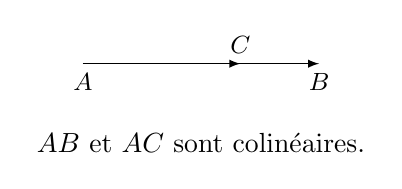
\begin{tikzpicture}[>=latex,scale=0.5]
            \draw[->] (0,0) node[below] {\small $A$} -- (6,0) node[below] {\small $B$};
            \draw[->] (0,0) -- (4,0) node[above] {\small $C$};
            \draw (3,-2) node{$\vect{AB}$ et $\vect{AC}$ sont colinéaires.};
        \end{tikzpicture}
    \end{center}
\end{Defi}

Dans un repère $\Oij$, on note $\binom x y$ les coordonnées de $\vect u$. Puisque $\vect v = k\vect u$ alors $\binom{kx}{ky}$ sont les coordonnées de $\vect v$. Peu importe le sens des vecteurs, on a :
$\PS u v = kx^2 + ky^2 = k(x^2 + y^2)$.
    \[\begin{array}{rcl}
        \norme{\vect u} \times \norme{\vect v} & = & \sqrt{(x^2 + y^2)} \times \sqrt{(kx)^2 + (ky)^2} \\
                                                                     & = & \sqrt{(x^2 + y^2) \times (k^2)(x^2 + y^2)} \\
                                                                     & = & \sqrt{k^2 \times (x^2 + y^2)^2} \\
                                                                     & = & \sqrt{k^2} \times \sqrt{(x^2 + y^2)^2} \\
                                                                     & = & \sqrt{k^2} \times (x^2 + y^2)
    \end{array}\]
Or, si $k \geq 0$ alors $\sqrt{k^2} = k$ et si $k \leq 0$, $\sqrt{k^2} = -k$. On obtient donc la propriété suivante :

\begin{Prop}
    Soient $\vect u$ et $\vect v$ deux vecteurs colinéaires.\par
    \begin{description}
        \item[$\vect u$ et $\vect v$ sont de même sens :] alors $\PS u v = \norme{\vect u} \times\norme{\vect v}$.
        \item[$\vect u$ et $\vect v$ sont de sens contraire :] alors $\PS u v = -\norme{\vect u} \times\norme{\vect v}$.
    \end{description}
\end{Prop}

\section{Projeté orthogonal}

\begin{Defi}
    On considère trois points $A$, $B$ et $C$.\par
    Le \ipt{projeté orthogonal} de $C$ sur la droite $(AB)$ est le point $H$ tel que :
    \[H \in (AB) \qetq (AB) \bot (CH).\]
    \begin{center}
        \begin{tikzpicture}[>=latex,scale=0.5]
            \draw (0,0) node[below] {\small $A$} -- (6,0) node[below] {\small $B$};
            \draw (0,0) -- (4,2) node[above] {\small $C$};
            \draw[dashed] (4,2) -- (4,0) node[below] {\small $H$} node {$\times$};
        \end{tikzpicture}
        \qquad
        \begin{tikzpicture}[>=latex,scale=0.5]
            \draw[dashed] (-4,0)--(0,0);
            \draw (0,0) node[below] {\small $A$} -- (6,0) node[below] {\small $B$};
            \draw (0,0) -- (-3,2) node[above] {\small $C$};
            \draw[dashed] (-3,2) -- (-3,0) node[below] {\small $H$} node {$\times$};
        \end{tikzpicture}
    \end{center}
\end{Defi}

\begin{Rmq}[s]
    \begin{itemize}
        \item Les vecteurs $\vect{AB}$ et $\vect{AH}$ sont colinéaires.
        \item Si $C \in (AB)$ alors $H$ et $C$ sont confondus : $H = C$.
        \item Si $(AC) \bot (AB)$ alors $A = H$ et si $(BC) \bot (AB)$ alors $H = B$.
    \end{itemize}
\end{Rmq}

\begin{Prop}
    On considère trois points $A$, $B$ et $C$ et on appelle $H$ le projeté orthogonal de $C$ sur la droite $(AB)$. Alors :
    \[\PS{AB}{AC} = \PS{AB}{AH} = \pm\norme{\vect{AB}} \times \norme{\vect{AH}}\] le signe dépendant du sens de $\vect{AH}$ par rapport à $\vect{AB}$.
\end{Prop}

\begin{Demo}
    Il suffit d'utiliser la relation de Chasles et la propriété \ref{Prop_PS} de la page \pageref{Prop_PS} :
    \[\begin{array}{rcl}
        \PS{AB}{AC} & = & \vect{AB} \cdot \vect{AH} + \vect{HC} \\
                              & = & \PS{AB}{AH} + \PS{AB}{HC} \\
                              & = & \PS{AB}{AH} + 0 \quad \text{puisque}\quad \vect{AB} \bot \vect{HC}
    \end{array}\]
\end{Demo}

Dans les configurations précédentes, on note $\alpha = \left(\vect{AB} \pv \vect{AC}\right)$.
    \begin{description}
        \item[\textbullet $\vect{AB}$ et $\vect{AH}$ sont de même sens :] les formules de trigonométrie dans le triangle $ACH$ rectangle en $H$ permettent d'affirmer que :
            \[AH = AC \times \cos \alpha.\]
        Ainsi, $\PS{AB}{AC} = AB \times AH = AB \times AC \cos \alpha$.
        \item[\textbullet $\vect{AB}$ et $\vect{AH}$ sont de sens contraire :] alors $\left(\vect{AC} \pv \vect{AH}\right) = \pi - \alpha$. Dans le triangle $ACH$ rectangle en $H$, les formules de trigonométrie permettent d'affirmer que :
            \[AH = AC \times \cos(\pi - \alpha) = -AC \times\cos(\alpha).\]
        Ainsi, $\PS{AB}{AC} = -AB \times AH = -AB \times (-AC \cos \alpha) = AB \times AC \cos \alpha$.
    \end{description}
    
\begin{Prop}
    Soient $\vect u$ et $\vect v$ deux vecteurs.\par
    \[\PS u v = \norme u \times\norme v \times \cos\left(\vect u , \vect v\right).\]
\end{Prop}

\begin{Rmq}
    Puisque $\cos \alpha$ = $-\cos\alpha$, on retrouve $\PS u v = \PS v u$.
\end{Rmq}

\begin{Exemple}
    On considère les points $A(1 \pv 1)$, $B(4 \pv 2)$ et $C(2 \pv 3)$.\par
    En arrondissant à l'unité, déterminer la mesure des angles du triangle $ABC$.
\end{Exemple}
    



\end{document}
